{\fontsize{12pt}{22pt} \textbf{Parametric Tests}\par}

\vspace{5mm}

Procedure:

1) find the test to perform

2) find the right estimator to use

3) deduce the reject region

4) compute the test statistic

5) retrieve quantiles of known distributions

\vspace{5mm}

Example 1: 

\vspace{5mm}

(\textit{inspired from example in Saporta p.325})

\vspace{5mm}

$X_1,...,X_n~(iid)\sim \mathbb{P_\theta}$

\vspace{5mm}

We want to analyze the mean. $m=a$?

\vspace{5mm}

1) find the test to perform

\vspace{5mm}

$
\left\{
    \begin{array}{ll}
        \mathcal{H}_0: \theta=a \\
        \mathcal{H}_1: \theta>a \\
    \end{array}
\right.
$

\vspace{5mm}

2) find the right estimator to use

\vspace{5mm}

Since we are testing the mean, we choose the empirical mean as \textbf{estimator} $\widehat{\theta}=\frac{1}{n}\sum{X_i}$

\vspace{5mm}

3) deduce the reject region

\vspace{5mm}

We fix $k$ for a rejection level $\alpha$. The rejection region is:

$Z=\{\widehat{\theta} \ge k\}$

\vspace{5mm}

We look for $k$ defined as such:

$\mathbb{P}_{\theta \in \Theta_0}(\widehat{\theta} \ge k)=\alpha$ => under $\mathcal{H}_0$, we reject the hypothesis when our estimator $\widehat{\theta}$ is above $k$

\textit{Intuitively, we want to keep our hypothesis if it's verified in most of the cases => under our hypothesis, there is a low probability that we are in the rejection region.}

\textit{Thus, if in real life we have a result that makes the hypothesis unverified, we reject the hypothesis. However, we have a risk of $\alpha$ that our hypothesis was correct and that we ended up in the rejection region by mistake.}

\vspace{5mm}

4) compute the test statistic

\vspace{5mm}

We center and reduce the estimator in order to get the Gaussian law and thus end up with known quantiles:

$\mathbb{P}_{\theta = a}(T \ge \frac{\sqrt{n} (k-a)}{\sqrt{\sigma^2}})=\alpha$ with $T \sim_{n \to \infty} \mathcal{N}(0,1)$

$T$ is the test statistic (\textcolor{red}{a test statistic is a random variable for which we know the law under $\mathcal{H}_0$})

\vspace{5mm}

5) retrieve quantiles of known distributions

\vspace{5mm}

Finally, $\frac{\sqrt{n} (k-a)}{\sqrt{\sigma^2}}=q_\alpha$ => we can find $k$ telling us when rejecting $\mathcal{H}_0$

\vspace{5mm}

\textcolor{gray}{We not looking at the average directly?}

=> the average can be influenced by the outliers and thus doesn't take into consideration extreme events.

\vspace{5mm}

\textcolor{gray}{How about the median?}

=> the median doesn't take into account the distribution / tendency of the values.

\vspace{5mm}

$\alpha$ is also called the p-value. The lower the p-value is, the less error we make in rejecting our hypothesis so the more significant the rejection is.

\textcolor{red}{p-value is the lowest error probability we want to make when rejecting our hypothesis.}

\vspace{5mm}

When performing OLS, our hypothesis is $\theta_{x1}=0$ so we reject it if the pvalue column is higher than our threshold. In the below OLS result, pvalues are displayed in column $P>|t|$. All variables are significant.

\begin{center}
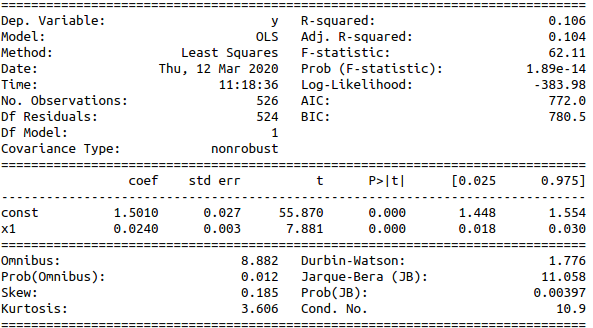
\includegraphics[scale=0.5]{OLS_pvalue.png}
\end{center}

\vspace{5mm}